\documentclass[border=10pt]{standalone}
\usepackage[svgnames]{xcolor}
\usepackage{amsmath}
\usepackage{pgfplots}
\pgfplotsset{compat=newest}
\usepackage[sfdefault]{FiraSans}
\usepackage{FiraMono}
\renewcommand*\familydefault{\sfdefault}
\begin{document}
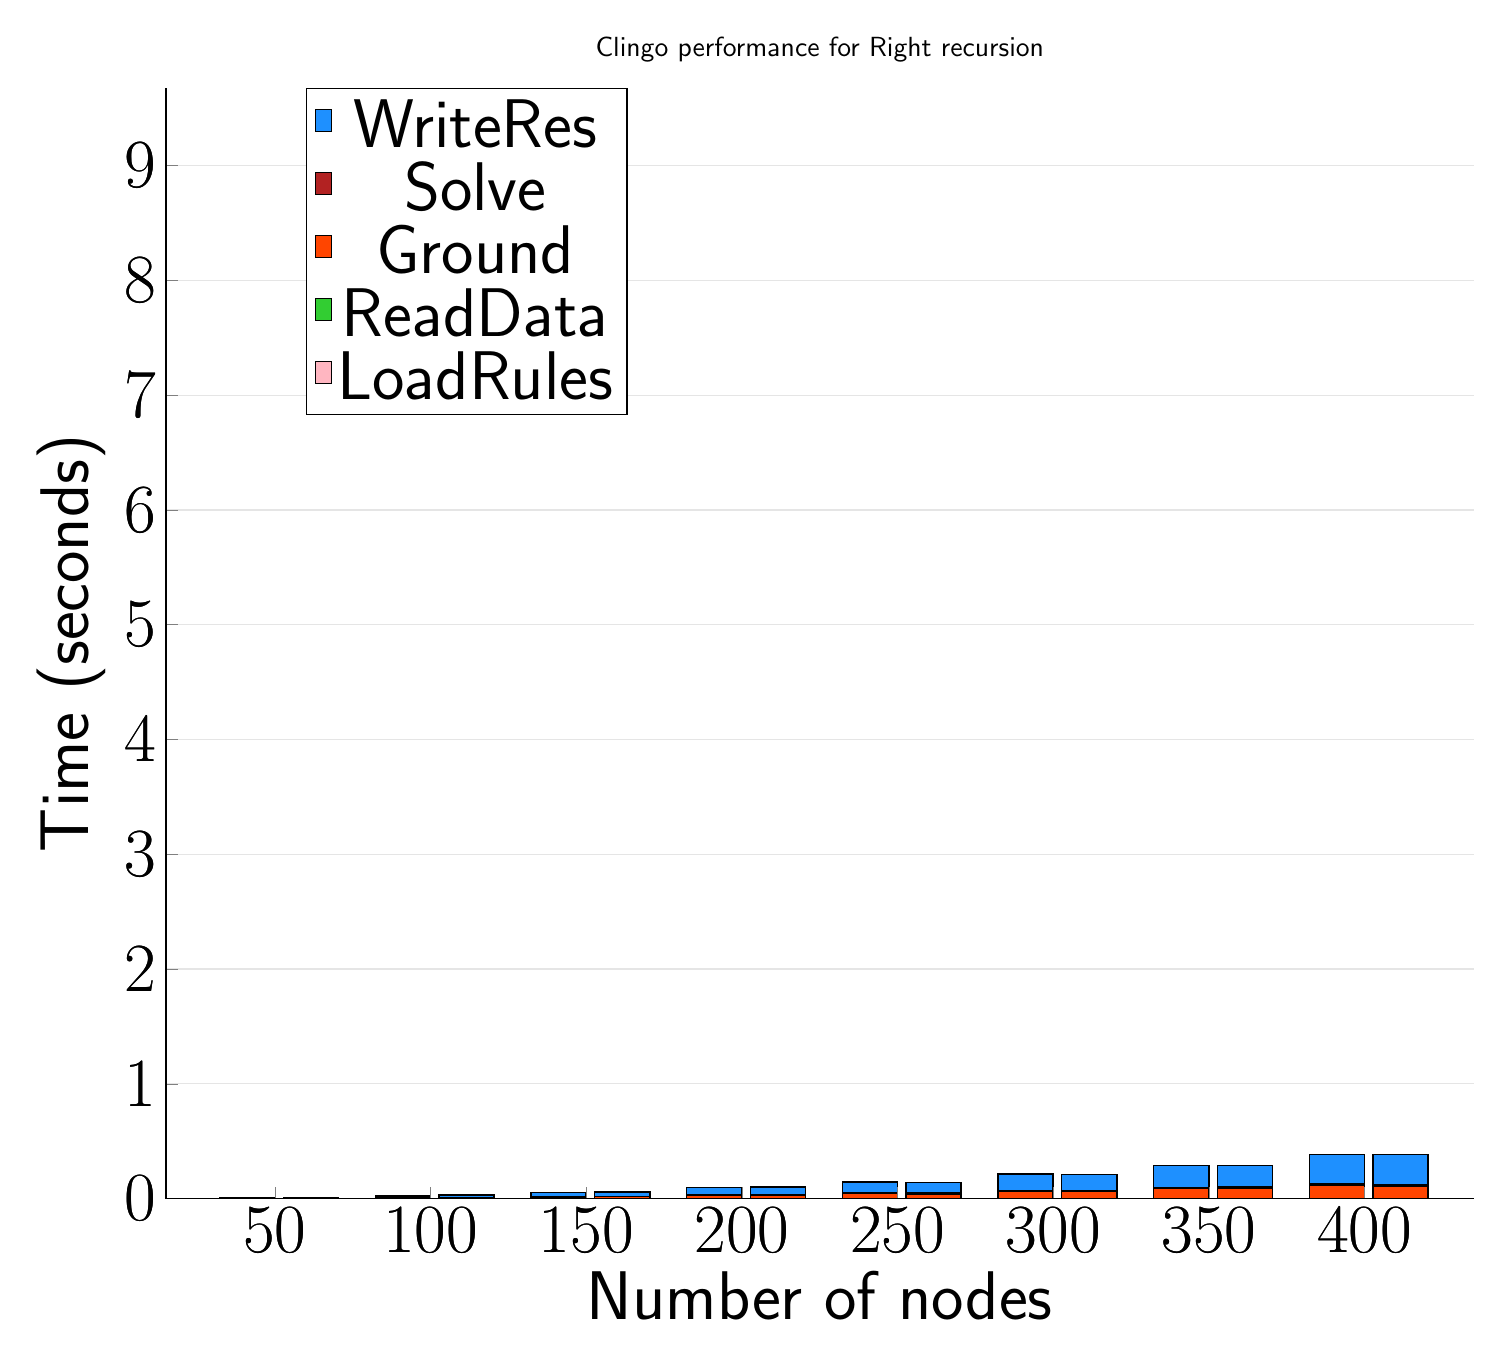
\begin{tikzpicture}
\begin{axis}[
   ybar stacked,
   title={Clingo performance for Right recursion},
   bar shift=-10pt,
   width=1.5\textwidth,
   bar width=0.7cm,
   ymajorgrids, tick align=inside,
   major grid style={draw=gray!20},
   xtick=data,
   ymin=0, ymax=9.677999997138977,
   axis x line*=bottom,
   axis y line*=left,
   enlarge x limits=0.1,
   legend style={
       at={(0.23, 1)},
       anchor=north,
       legend columns=1,
       font=\Huge,
   },
   ylabel={Time (seconds)},
   xlabel={Number of nodes},
   label style={font=\Huge},
   tick label style={font=\Huge},
]
\addlegendimage{fill=DodgerBlue, draw=black, line width=0.2pt}
\addlegendentry{WriteRes}
\addlegendimage{fill=FireBrick, draw=black, line width=0.2pt}
\addlegendentry{Solve}
\addlegendimage{fill=OrangeRed, draw=black, line width=0.2pt}
\addlegendentry{Ground}
\addlegendimage{fill=LimeGreen, draw=black, line width=0.2pt}
\addlegendentry{ReadData}
\addlegendimage{fill=LightPink, draw=black, line width=0.2pt}
\addlegendentry{LoadRules}
\addplot +[fill=LightPink, draw=black, line width=0.5pt] coordinates {
    (50, 0.0)
    (100, 0.0)
    (150, 0.0)
    (200, 0.0)
    (250, 0.0)
    (300, 0.0)
    (350, 0.0)
    (400, 0.0)
};
\addplot +[fill=LimeGreen, draw=black, line width=0.5pt] coordinates {
    (50, 0.0)
    (100, 0.0)
    (150, 0.0)
    (200, 0.0009999990463256836)
    (250, 0.0009999990463256836)
    (300, 0.0019999980926513673)
    (350, 0.0)
    (400, 0.0019999980926513673)
};
\addplot +[fill=OrangeRed, draw=black, line width=0.5pt] coordinates {
    (50, 0.0019999980926513673)
    (100, 0.008000016212463379)
    (150, 0.015000033378601074)
    (200, 0.02799999713897705)
    (250, 0.043000006675720216)
    (300, 0.06099996566772461)
    (350, 0.08699998855590821)
    (400, 0.11299998760223388)
};
\addplot +[fill=FireBrick, draw=black, line width=0.5pt] coordinates {
    (50, 0.0009999990463256836)
    (100, 0.0019999980926513673)
    (150, 0.0019999980926513673)
    (200, 0.0019999980926513673)
    (250, 0.005999994277954101)
    (300, 0.007999992370605469)
    (350, 0.012000012397766113)
    (400, 0.012000036239624024)
};
\addplot +[fill=DodgerBlue, draw=black, line width=0.5pt] coordinates {
    (50, 0.005000019073486328)
    (100, 0.01399998664855957)
    (150, 0.03599998950958252)
    (200, 0.06399998664855958)
    (250, 0.09600000381469727)
    (300, 0.14200007915496826)
    (350, 0.19099996089935303)
    (400, 0.2549999475479126)
};
\end{axis}
\begin{axis}[
   ybar stacked,
   bar shift=13pt,
   width=1.5\textwidth,
   bar width=0.7cm,
   ymajorgrids, tick align=inside,
   major grid style={draw=none},
   xtick=data,
   ymin=0, ymax=9.677999997138977,
   axis x line*=none,
   axis y line*=none,
   enlarge x limits=0.1,
   label style={font=\Huge},
   tick label style={font=\Huge},
]
\addplot +[fill=LightPink, draw=black, line width=0.5pt] coordinates {
    (50, 0.0)
    (100, 0.0)
    (150, 0.0)
    (200, 0.0)
    (250, 0.0)
    (300, 0.0)
    (350, 0.0)
    (400, 0.0)
};
\addplot +[fill=LimeGreen, draw=black, line width=0.5pt] coordinates {
    (50, 0.0)
    (100, 0.0)
    (150, 0.0)
    (200, 0.0)
    (250, 0.0)
    (300, 0.0)
    (350, 0.0)
    (400, 0.0)
};
\addplot +[fill=OrangeRed, draw=black, line width=0.5pt] coordinates {
    (50, 0.0)
    (100, 0.009999999999999997)
    (150, 0.019999999999999997)
    (200, 0.030000000000000006)
    (250, 0.03999999999999999)
    (300, 0.06000000000000001)
    (350, 0.08799999999999998)
    (400, 0.11000000000000001)
};
\addplot +[fill=FireBrick, draw=black, line width=0.5pt] coordinates {
    (50, 0.0)
    (100, 0.0)
    (150, 0.0)
    (200, 0.0)
    (250, 0.010000000000000009)
    (300, 0.009999999999999995)
    (350, 0.011999999999999993)
    (400, 0.012000000000000005)
};
\addplot +[fill=DodgerBlue, draw=black, line width=0.5pt] coordinates {
    (50, 0.009999999999999997)
    (100, 0.020000000000000007)
    (150, 0.038)
    (200, 0.06999999999999998)
    (250, 0.08999999999999998)
    (300, 0.139)
    (350, 0.18999999999999997)
    (400, 0.25999999999999995)
};
\end{axis}
\end{tikzpicture}

\end{document}
